\documentclass[11pt, a4paper]{article}
\usepackage[utf8]{inputenc}
\usepackage[russian]{babel}
\usepackage{amsmath}
\usepackage{amsfonts}
\usepackage{amssymb}
\usepackage{setspace}
\usepackage{changepage}
\usepackage{graphicx}
\DeclareGraphicsExtensions{.png,.pdf,.jgp}
\usepackage{caption}
\usepackage{ccaption}
\captionsetup[figure]{labelformat=empty}

\textwidth=18cm
\oddsidemargin=-1cm
\evensidemargin=-1cm
\topmargin=-2.5cm
\textheight=32cm
\linespread{0.8}

\begin{document}
	\Large
	
	\begin{adjustwidth}{1.5cm}{}
		172 
		\vspace*{-14pt}
		\begin{center}
			III. ЗАКОНЫ СОХРАНЕНИЯ
		\end{center}
		\vspace*{-7pt}
		
		\hspace*{-0.6cm}\rule{16.5cm}{0.5pt}
	
		\begin{itemize}
			\item В каких случаях законом сохранения импульса системы можно пользоваться и при наличии внешних сил?
			\item Какие преимущества дает использование закона сохранения импульса по сравнению с динамическим подходом?
			\item Когда на тело действует переменная сила $F(t)$, ее импульс определяется правой частью формулы (5) — интегралом от $F(t)$ по промежутку времени, в течение которого она действует. Пусть нам дан график зависимости $F(t)$ (рис. 109). Как по этому графику определить импульс силы для каждого из случаев \itа \rmи \itб?
		\end{itemize}
		
		\noindent\textbf{\S 30. Центр масс. Реактивное движение}
		\vspace{0.4cm}
		
		\noindent Когда мы имеем дело с системой частиц, удобно найти такую точку — \itцентр масс\rm, которая характеризовала бы положение и движение этой системы как целого. В системе из двух одинаковых частиц такая точка С, очевидно, лежит посередине между ними (рис. 110\itа\rm). Это ясно из соображений симметрии: в однородном и изотропном пространстве эта точка выделена среди всех остальных, ибо для любой другой точки А, расположенной ближе к одной из частиц, налется симметричная ей точка В, расположенная		
	
		\begin{figure}[h]
			\hspace{1.5cm}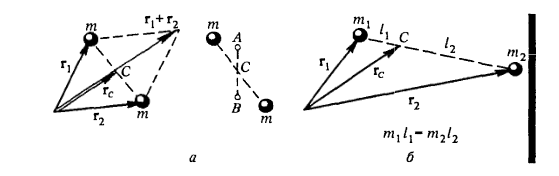
\includegraphics[scale=0.8]{graphic}
			\begin{adjustwidth}{1.5cm}{}
				\hangcaption{Рис. 110. Центр масс двух одинаковых частиц находится в точке $C$ с радиусом-вектором $r_C=(r_1+r_2)/2$ (\itа\rm); центр масс двух частиц с разной массой делит отрезок между ними в отношении, обратно пропорциональном массам чатиц (\itб\rm)}
			\end{adjustwidth}
		\end{figure}
		
		
		
		\noindentближе ко второй частице. Очевидно, что радиус-вектор $r_C$ точки $C$ равен полусумме радиусов-векторов $r_1$ и $r_2$ одинаковых частиц (рис. 110\it a\rm): $r_C = (r_1 + r_2)/2$. Другими словами, $r_C$ представляет собой обычное среднее значение векторов $r_1$ и $r_2$.
		
		\vspace{0.4cm}
		
		\noindent\textbf{Определение центра масс.} Как обобщить это определение на случай двух частиц с разными массами $m_1$ и $m_2$? Можно ожидать, что наряду с геометрическим центром системы, радиус-вектор которого по-прежнему равен полусумме $(r _1+ r _2)/2$, будет играть определенную роль точка, положение которой определяется распределени-
		
		
	\end{adjustwidth}
	
\end{document}